\subsubsection*{Problem definition}

The non-linear Freundlich isotherm is often used to describe real sorption processes. Therefore, in this example, the transport process by including the Freundlich isotherm is calculated in the same way as in the precedent example (same model and boundary conditions). As there exists no opportunity to calculate analytically the solute transport with non-linear sorption, the results of the simulation have to be compared with solutions of the transport equation with linear sorption in order to evaluate the simulation results.

\textsl{Assumptions}

\begin{tabbing}
Component: \= non-linear sorption (Freundlich isotherm), no decay \\
Aquifer: \> homogeneous, saturated, stationary flow \\
\end{tabbing}

\subsubsection*{Model set-up of the 1~D numerical model}

See chapter \ref{sec:decay}

The soil parameters are the same as listed in table \ref{tab51}(except decay). For the different simulation runs the Freundlich-sorption coefficients (K$_1$) are varied in the same way as the K$_D$-values that are listed in table \ref{tab53}. The exponent K$_2$ was constant with a value of 1.

\subsubsection*{Evaluation method}
The dependence of sorbed molecules on the amount of molecules in dilution is given by equation \ref{eq59}. The concentration distribution at a special point in time and over a given distance cannot be calculated analytically by equation \ref{eq53} when a non-linear sorption process is assumed. A possibility to test the correctness of the simulation results for transport with Freundlich sorption is to choose values of distribution coefficients in order to create a concentration distribution which is approximately linear and must therefore almost be equal to the results of transport by use of the Henry isotherm.

\subsubsection*{Results}

As the values for the Freundlich coefficients were chosen in that way, that the concentration distribution between sorbed and solute concentrations is almost linear, the results of the simulation runs have to be equal to the results that are obtained by using the linear Henry isotherm. In figure \ref{fig54} the concentration distribution of the solute over the model length of 100~m is shown. As the concentrations of the transport simulation by using the Freundlich isotherm match those of the simulation runs with linear sorption, these results for non-linear sorption are reasonable. Additionally to this test, the values for the constant K$_2$ were changed to 0.8 in order to prove a difference between linear and non-linear sorption. The results of the comparison are shown in figure \ref{fig55}. These numerical results show the effect of the application of a non-linear sorption isotherm: the higher the influence of sorption (large value of sorption coefficient K$_D$ resp. K$_1$) the higher the difference of solute concentration values between non-linear and linear sorption. However, the results for both isotherms were not evaluated quantitatively.

\begin{figure}[htbp]
\centering
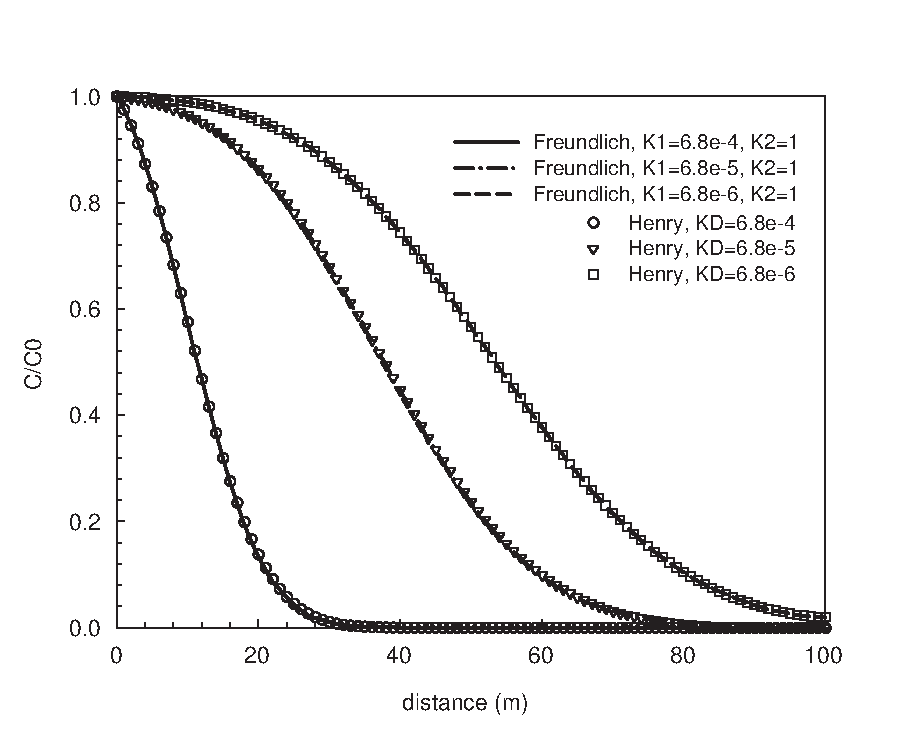
\includegraphics[width=0.8\textwidth]{C/figures/fig54.EPS}
\caption{Concentration distribution after 100~d (Freundlich compared to Henry sorption)}
\label{fig54}
\end{figure}

\begin{figure}[htbp]
\centering
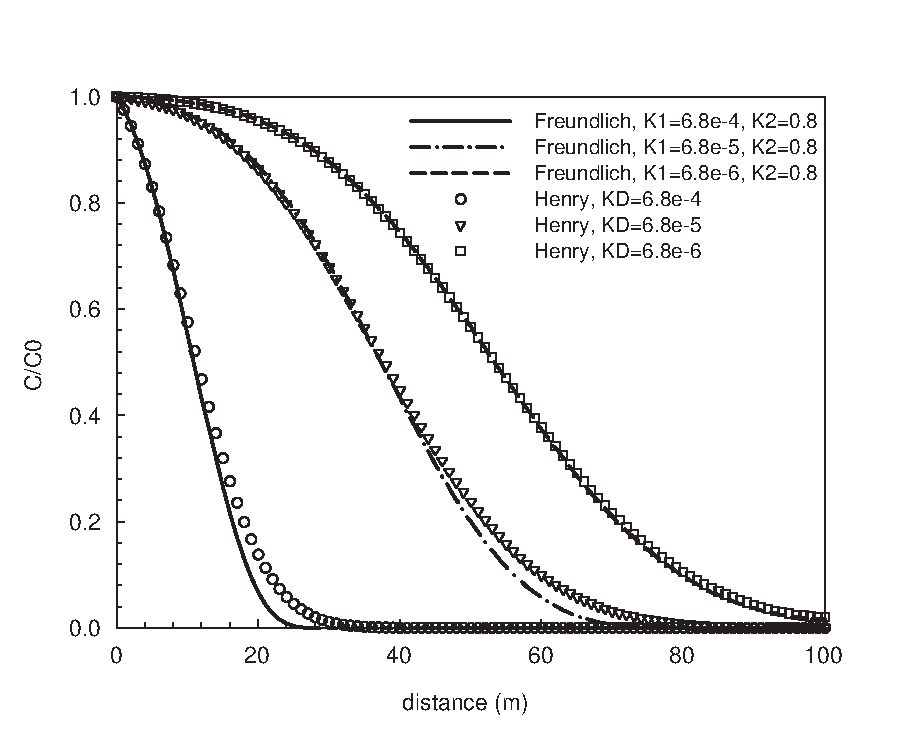
\includegraphics[width=0.8\textwidth]{C/figures/fig55.EPS}
\caption{Different concentration distributions after 100~d (Freundlich compared to Henry sorption)}
\label{fig55}
\end{figure}

\begin{tabular}{|l|l|l|}
\hline
Benchmark & Problem type	& Path in benchmark deposit \\
\hline	
hc\_sorp\_Freundl\_1D	& HC	& benchmarks $\backslash$HC$\backslash$Sorption$\backslash$Freundlich \\
\hline	
\end{tabular}

